\section{La hidrografía de Europa}

\begin{figure}[!ht]
    \centering
    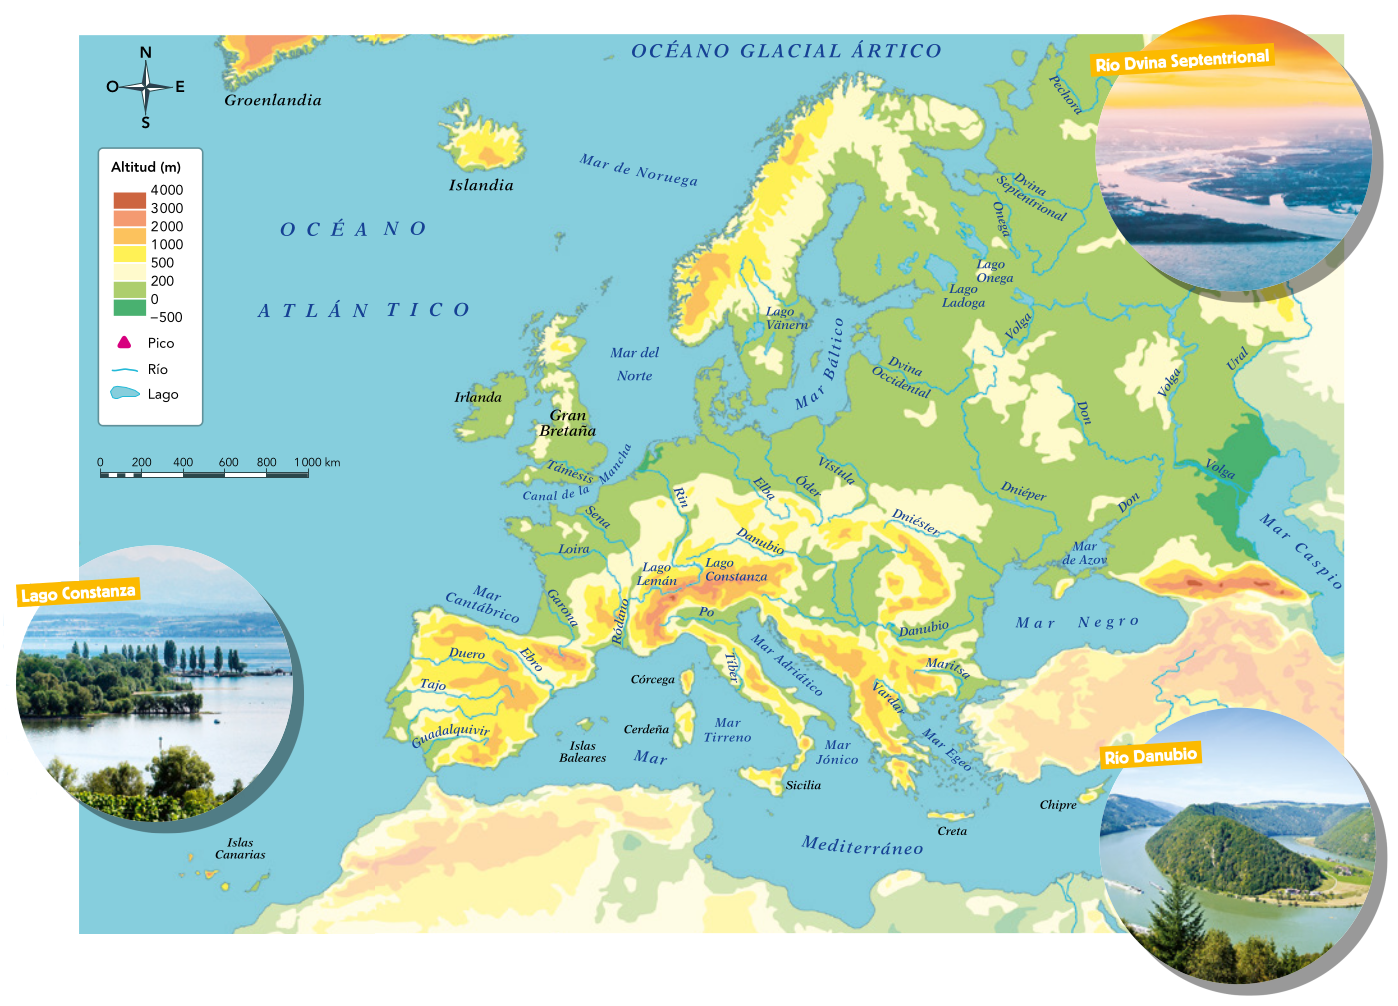
\includegraphics[width=1\linewidth]{Tema2/10_Rios_Europa.png}
    \caption{Hidrografía de Europa}
    \label{fig:hidrografia-europa}
\end{figure}

\subsection{Los océanos y los mares}

Europa está rodeada de océanos y mares. En las costas del norte y el oeste del continente, tenemos los océanos Glacial Ártico y Atlántico.

\vspace{3mm}
Los mares que bañan las costas de Europa son el de Noruega, del Norte, Báltico, Cantábrico, el Mediterráneo, el Adriático, etcétera. También hay dos mares interiores, el mar Negro y el mar Caspio.

\subsection{Los lagos europeos}

Los lagos en Europa son muy abundantes.

\begin{enumerate}
    \item En el norte destacan el Ladoga y el Onega.
    \item Los lagos centroeuropeos como el Lemán y el Constanza se encuentran a lo largo de los Alpes.
    \item Los lagos mediterráneos son de menor tamaño.
\end{enumerate}

\subsection{Los ríos europeos}

Las características de los ríos europeos están determinadas por el relieve y el clima.

\subsubsection{Los ríos de las vertientes ártica y atlántica}

Son ríos largos que suelen tener cuencas muy extensas.

\begin{itemize}
    \item Los ríos que desembocan en el Glacial Ártico son caudalosos e irregulares, como el Dvina Septentrional.
    \item Los ríos que desembocan en el océano Atlántico son caudalosos y regulares. Destacan el Vístula, el Rin, el Sena y el Loira.
\end{itemize}

\subsubsection{Los ríos de la vertiente mediterránea}

Estos suelen ser cortos e irregulares, como el Po.

\subsubsection{Los ríos que desembocan en los mares interiores}

Estos ríos son largos, caudalosos y navegables. Destaca el Danubio, que vierte sus aguas en el mar Negro y el Volga, que es el río más largo de Europa y desemboca en el mar Caspio.